
\section{Capítulo: Análisis}
\label{sec:cap5}
A continuacón se presenta un análisis, comparación y seleccción de las

herramientas y tecnologías a utilizar en el desarrollo de este proyecto.
Asimismo, se exponen las razones que justifican su elección 
considerando aspectos técnicos, económicos y de disponibilidad 
con base en las necesidades del sistema, evaluando las ventajas y desventajas 
de cada alternativa, así como su integración.
\subsection{Análisis de tecnologías del Módulo 1}
\label{sec:mod1}
En esta sección se presentan el análisis, la comparación y la selección de los sensores, 
así como del microcontrolador que se implementarán en el Módulo 1 del proyecto. 
Dicha evaluación se lleva a cabo mediante tablas comparativas entre 
las distintas opciones disponibles en el mercado que cumplen con los
requerimientos funcionales establecidos.

A continuación, se describen los componentes principales que integran el Módulo 1:
\subsubsection{Sensor de pH}
Para medir el pH del kéfir de leche durante la fermentación, se
utilizará un sensor de pH analógico. Este sensor debe ser capaz de proporcionar
una salida de voltaje proporcional al valor de pH medido.
Para la selección del sensor de pH, se consideraron los siguientes
criterios en base a los requeriminetos funcionales \ref{it:RF01} del
proyecto:
\begin{itemize}
    \item \textbf{No contaminante:} El sensor debe ser adecuado para su uso en
    líquidos, en especial, en fermentaciones y no debe estar hecho de un material que pueda
    contaminar el kéfir por lo que es recomendado que este hecho de algun polimero de grado alimenticio, vidiro o de ceramica.
    \item \textbf{Rango de medición:}El sensor debe cubrir el rango de pH esperado durante
    la fermentación del kéfir de leche, que típicamente varía entre 6.8(inicial) y
    4.6(final).
    \item \textbf{Precisión:}El sensor debe tener una precisión adecuada para detectar
    cambios pequeños en el pH, idealmente con una precisión de ±0.1 pH.
    \item \textbf{Salida:}Se consideraron sensores con conectores estándar (como BNC)
    para facilitar una salida digital y una conexión con el microcontrolador.
    \item \textbf{Temperatura de operación:}El sensor debe ser capaz de operar en el
    rango de temperatura esperado durante la fermentación (18-30 °C).
    \item \textbf{Disponibilidad y costo:}Se consideraron sensores que sean fácilmente
    adquiribles y con un costo razonable para el proyecto.
\end{itemize}
A continuación, se presenta un análisis comparativo de los diferentes sensores de pH considerados para el proyecto:


\begin{landscape}
\begin{table}[h!]
    \centering
    \small
    \caption{Sensores de pH.}
% Anchos de columna reducidos para encoger la tabla horizontalmente.
\begin{tabular}{|m{1.6cm}|m{1cm}|m{1.3cm}|m{2cm}|m{1cm}|m{1cm}|m{1.8cm}|m{1.5cm}|m{1.5cm}|m{1.4cm}|m{1.4cm}|m{2.0cm}|}
\hline
% FILA DE ENCABEZADOS
\textbf{Modelo} & 
\textbf{Rango} & 
\textbf{Volta- je} & 
\textbf{Referencia} & 
\textbf{Pre- cisión} & 
\textbf{Tiem- po de Respuesta} & 
\textbf{Tempe- ratura de operación °C} & 
\textbf{Cuerpo} & 
\textbf{Punta} & 
\textbf{Tipo de Salida} & 
\textbf{Precio (MXN)} & 
\textbf{Imagen} \\ 
\hline
% DATOS - Heredan el tamaño \small
Hanna Instrume- nts-FC200B\cite{zotero-item-24} & 0 a 12pH & 3.3V-5.5V & Ag/AgC (Plata/cloruro de plata) & 0,1 & N/A & 0 a 50°C & PVDF & Cónica de vidrio & BNC & \$5233.92 &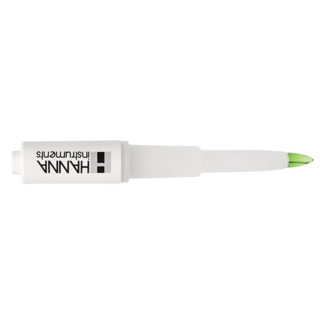
\includegraphics[width=20mm]{./Imagenes/Módulo1/pH/S1.jpg} \\ \hline

Milwaukee SE-220\cite{ElectronicsKft.2019} & 0 a 14pH & 3.3V-5.5V & doble unión Ag/AgC & 0,02 & N/A & -5 a 70°C & Resina-PEI & esférica & BNC & \$1762 & 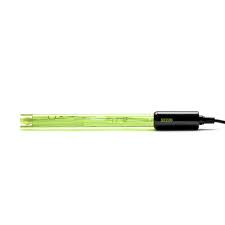
\includegraphics[width=20mm]{./Imagenes/Módulo1/pH/images.jpeg} \\ \hline

Atlas Científic-ENV-40-pH \cite{zotero-item-35} & 0 a 14pH & 3.3V-5.5V & doble unión Ag/AgC & 0,001 & 1 seg. & 5 - 99°C & Polica- rbonato & esférica & BNC & \$3000-4000 & 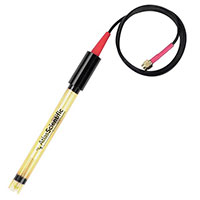
\includegraphics[width=20mm]{./Imagenes/Módulo1/pH/MFG_ENV-40-pH_primary_sml.jpg} \\ \hline

Atlas Científic-ENV-30-pH \cite{zotero-item-33} & 2 a 12pH & 3.3V-5.5V & Ag/AgC & 0.1 & 4 seg. & 0-60°C & Polica- rbonato & esférica & BNC & \$1000-2000 & 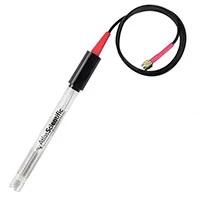
\includegraphics[width=20mm]{./Imagenes/Módulo1/pH/MFG_ENV-30-pH _primary_sml.jpg} \\ \hline

PH-E201C \cite{zotero-item-47} & 0 a 14pH & 5V & Ag/AgCl & 0.02 & 5 seg. & 0-80°C & Polica- rbonato & esférica & BNC & \$250-500 & 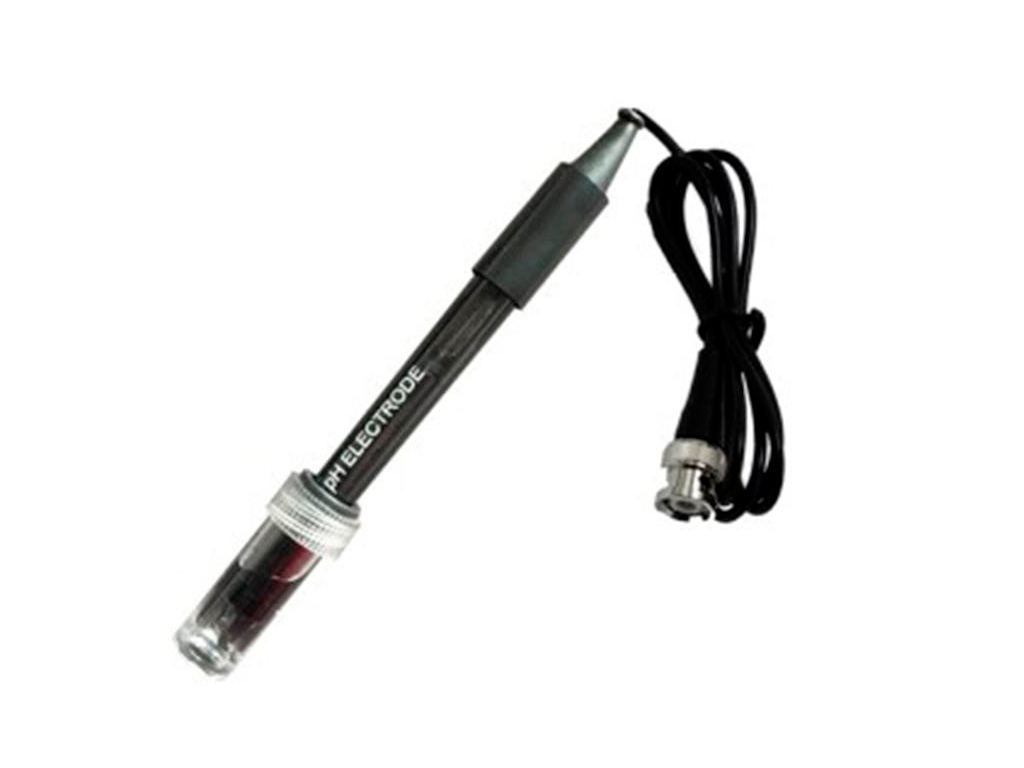
\includegraphics[width=20mm]{./Imagenes/Módulo1/pH/electrodo-para-medición-de-ph-e201c.jpg} \\ \hline
\end{tabular}

\label{tab:sensorespH}
\end{table}
\end{landscape}

Tras un análisis comparativo detallado de los sensores presentados en 
la \cref{tab:sensorespH}, se determinó que el electrodo
PH-E201C \cite{zotero-item-47} representa la opción más viable
para su integración en el proyecto. Si bien los modelos alternativos 
satisfacen la mayoría de los requerimientos funcionales, el PH-E201C 
ofrece un equilibrio superior entre desempeño técnico y viabilidad económica. 
Este sensor destaca por su elevada precisión de $0.02$\,unidades de pH y un 
tiempo de respuesta de $5$\,segundos. Adicionalmente, su costo accesible y 
amplia disponibilidad en el mercado lo consolidan como la solución más 
conveniente y eficiente frente a las alternativas de mayor precio.

\subsubsection{Sensor de Temperatura}
Para medir la temperatura del kéfir de leche durante la fermentación, se
utilizará un sensor de temperatura digital. Este sensor debe ser capaz de
proporcionar una lectura precisa de la temperatura en grados Celsius.
Para la selección del sensor de temperatura, se consideraron los siguientes
criterios en base a los requeriminetos funcionales \ref{it:RF01} del
proyecto:
\begin{itemize}
    \item \textbf{No contaminante:} El sensor debe ser adecuado para su uso en
    líquidos, en especial, en fermentaciones y no debe estar hecho de un material que pueda
    contaminar el kéfir por lo que es recomendado que este hecho de acero inoxidable de grado alimenticio.
    \item \textbf{Rango de medición:} El sensor debe cubrir el rango de temperatura
    esperado durante la fermentación del kéfir de leche, que típicamente varía entre
    18 y 30 °C.
    \item \textbf{Precisión:} El sensor debe tener una precisión adecuada para detectar
    cambios pequeños en la temperatura, idealmente con una precisión de ±0.5 °C.
    \item \textbf{Salida:} Se consideraron sensores con salida digital (como I2C o
    1-Wire) para facilitar la integración con el microcontrolador.
    \item \textbf{Disponibilidad y costo:} Se consideraron sensores que sean fácilmente
    adquiribles y con un costo razonable para el proyecto.
\end{itemize}
A continuación se presentan la tabla diferentes sensores de temperatura
considerados para el proyecto:

\begin{table}[h!]
    \centering
    \caption{sensores de temperatura.}
    \resizebox{\textwidth}{!}{
\begin{tabular}{|m{2.5cm}|m{2.5cm}|m{1.8cm}|m{2.5cm}|m{3.5cm}|m{2cm}|m{2cm}|m{2cm}|}
\hline
\textbf{Modelo}  & \textbf{Rangos de medición} & \textbf{Voltaje} & \textbf{Material} & \textbf{Error} & \textbf{Tipo de salida} & \textbf{Precio (MXN)} & \textbf{Imagen} \\ \hline
DS18B20\cite{zotero-item-78} & –55 °C a 125 °C & 3.3–5.5 V & Acero inoxidable & \begin{tabular}[c]{@{}c@{}}–10 °C a 85 °C\\ ±0.5 °C\end{tabular} & 1-Wire & \$50–150 & 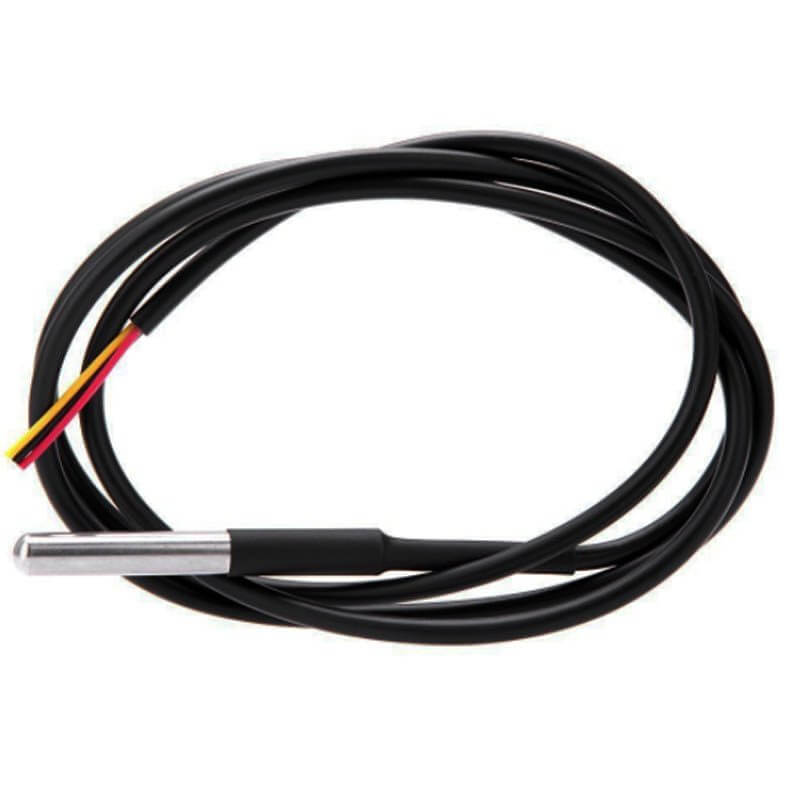
\includegraphics[width=20mm]{./Imagenes/Módulo1/Temperatura/t1.jpg} \\ \hline
E52-CA6DN 4M\cite{zotero-item-45} & 0–350 °C & 3.3–5.5 V & Acero inoxidable & \begin{tabular}[c]{@{}c@{}}0–333 °C\\ ±2.5 °C\end{tabular} & 1-Wire & \$2104 & 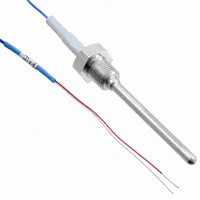
\includegraphics[width=20mm]{./Imagenes/Módulo1/Temperatura/t2.jpg} \\ \hline
\end{tabular}
    }
\label{tab:sensoresTemp}
\end{table}

Con base en los sensores presentados en la \cref{tab:sensoresTemp}, 
el sensor DS18B20 \cite{zotero-item-78} se integra mucho mejor al proyecto a diferencia de los otros sensores,
ya que presenta un índice de error de solo +/-0.5C combinada con su bajo coste lo convierte en la elección más eficiente.

\subsubsection{Sensor de $CO_{2}$}
Para medir la concentración de dióxido de carbono ($CO_{2}$) en el ambiente
circundante al kéfir de leche durante la fermentación, se utilizará un
sensor de $CO_{2}$. Este sensor debe ser capaz de proporcionar una lectura precisa
de la concentración de $CO_{2}$ en partes por millón (ppm).
Para la selección del sensor de $CO_{2}$, se consideraron los siguientes
criterios en base a los requerimietos funcionales \ref{it:RF01} del
proyecto:
\begin{itemize}
    \item \textbf{Rango de medición:} El sensor debe cubrir el rango de concentración
    de $CO_{2}$ esperado durante la fermentación del kéfir de leche, que típicamente varía
    entre 0 y 5000 ppm.
    \item \textbf{Precisión:} El sensor debe tener una precisión adecuada para detectar
    cambios pequeños en la concentración de $CO_{2}$, idealmente con una precisión de ±50 ppm.
    \item \textbf{Salida:}Se consideraron sensores con salida digital (como I2C o
    UART) para facilitar la integración con el microcontrolador.
    \item \textbf{Temperatura de operación:} El sensor debe ser capaz de operar en el
    rango de temperatura esperado durante la fermentación (18-30 °C).
    \item \textbf{Disponibilidad y costo:} Se consideraron sensores que sean fácilmente
    adquiribles y con un costo razonable para el proyecto.
\end{itemize}
A continuación se presentan en la \cref{tab:sensoresCO2} diferentes sensores de $CO_{2}$
considerados para el proyecto:


\begin{table}[h!]
    \centering
    \small % Tamaño de fuente pequeño para que quepa
    \caption{Sensores de $CO_{2}$}
 \resizebox{\textwidth}{!}{
% Definición de 7 columnas (m{ancho}) para el texto/datos + 1 columna de imagen = 8 COLUMNAS TOTALES
\begin{tabular}{|m{2.5cm}|m{2.5cm}|m{1.8cm}|m{2.5cm}|m{3.5cm}|m{2cm}|m{2cm}|} 
\hline
% LÍNEA DEL ENCABEZADO CORREGIDA (sin espacios innecesarios dentro de \$)
\textbf{Sensor} & \textbf{Precisión} & \textbf{Rango de medición} & \textbf{Temp. de operación °C} & 
\textbf{Voltaje / Consumo} & \textbf{Precio aprox. (MXN)} & \textbf{Imagen} \\ 
\hline
% Filas de datos (revisadas)
MQ-135\cite{zotero-item-48} & N/A & 10-1000 ppm (estimado, otros gases) & -20 a +50°C & 5 V & \$100-200 & 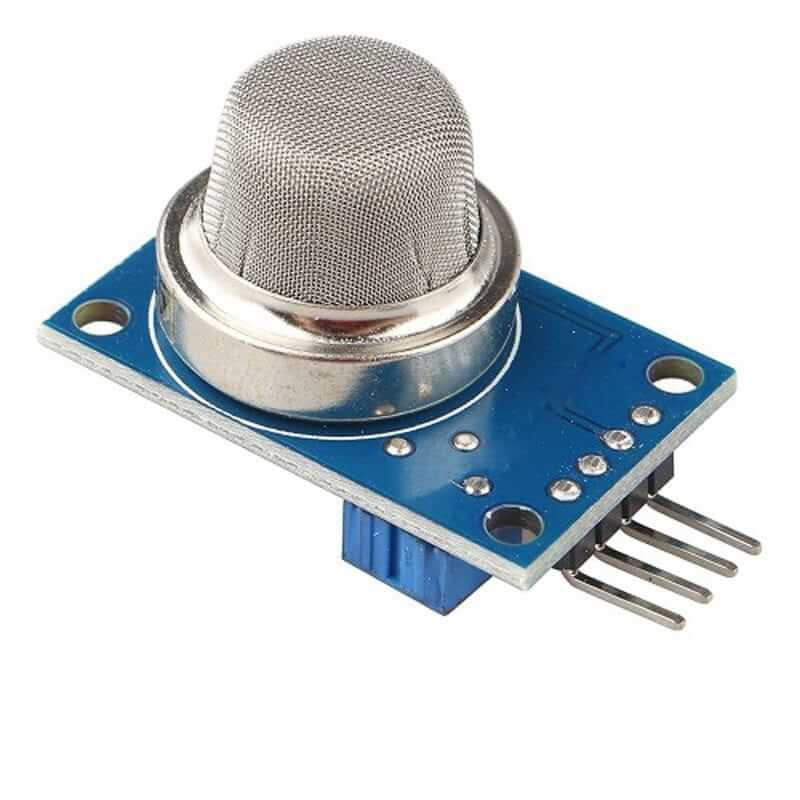
\includegraphics[width=20mm]{./Imagenes/Módulo1/Gas/mq135.jpg}\\ \hline

MH-Z19 / MH-Z19B\cite{zotero-item-50}& +/-(50ppm+5\%) & 400-10000 ppm & -10 a 50°C & 3.6-5.5 V & \$700-1700 & 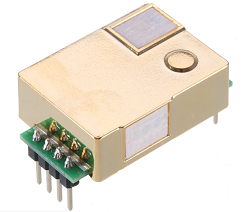
\includegraphics[width=20mm]{./Imagenes/Módulo1/Gas/HX-Z19.jpg} \\ \hline

SCD30 (Sensirion)\cite{zotero-item-52} &+/- (30ppm+3\%)  & 0-40000 ppm & 0 a 50°C & 3.3-5.5 V & \$780-1500 & 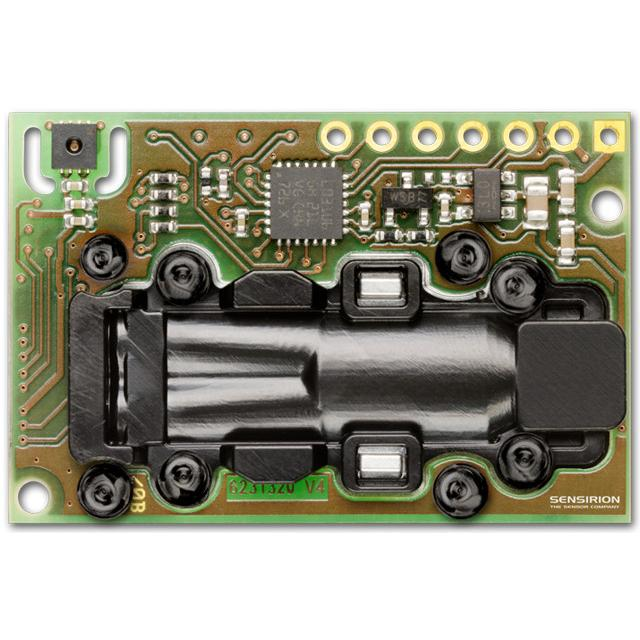
\includegraphics[width=20mm]{./Imagenes/Módulo1/Gas/scd30-5.jpg} \\ \hline

MG-811\cite{zotero-item-54} & +/- (30ppm+5\%)  & 350-10000 ppm & 20 a 50°C & 5-6 V& \$600-740 & 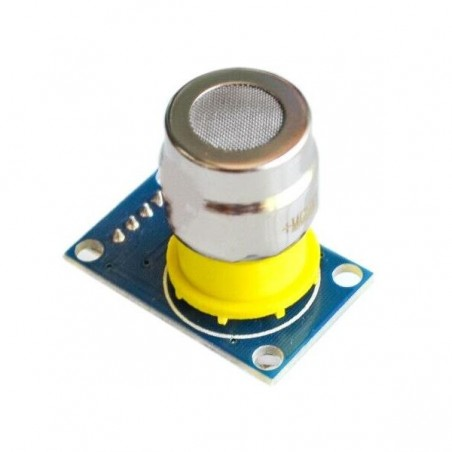
\includegraphics[width=20mm]{./Imagenes/Módulo1/Gas/md-mg81.jpg} \\ \hline
\end{tabular}
    }
    \label{tab:sensoresCO2}
\end{table}

Uno de los par\'ametros m\'as dif\'iciles de medir en la fermentaci\'on es 
el \textbf{${CO}_{2}$}. Dado que la fermentaci\'on del k\'efir libera grandes 
cantidades de este gas, se requiere un sensor con una excelente precisi\'on y un 
amplio rango de medici\'on. Con base en los sensores presentados en la  \cref{tab:sensoresCO2},
el sensor \textbf{MG-811} \cite{zotero-item-54} es la mejor opci\'on para el proyecto.
Esto se debe a que presenta un \'indice de error de solo +/-(30ppm+3\%) y por su rango de 
medici\'on . Aunque no es el m\'as barato, su especializaci\'on en 
la medici\'on de ${CO}_{2}$ evita los problemas de precisi\'on que tendr\'ian otros sensores.
\newline
\newline

Con el propósito de seleccionar el microcontrolador
adecuado, resulta indispensable evaluar previamente un 
conjunto de criterios técnicos; lo anterior permitirá analizar
con precisión las capacidades, prestaciones y limitaciones de cada alternativa considerada.

\subsubsection{Formato de Datos}
La elección del formato de datos es un aspecto crítico en el diseño del sistemas 
, ya que influye directamente en la eficiencia, la interoperabilidad y 
la escalabilidad del sistema. Con base en los formatos analizados en la 
\cref{tab:datos} y los requerimientos funcionales \ref{it:RF01}, se identifica a JSON (JavaScript Object Notation)
como la opción más adecuada esto debido a que permite estructurar datos de 
manera jerárquica, agrupando valores y metadatos en objetos anidados, lo que facilita la integración 
entre los módulos del sistema, características que cumplen con los requerimientos funcionales de interoperabilidad, 
eficiencia y escalabilidad.
En contraste, otros formatos presentan limitaciones significativas. CSV, aunque simple y compacto, carece de anidamiento 
y contexto, lo que lo hace inadecuado para datos complejos o flexibilidad en su estructura, ya que cualquier 
cambio en los datos implica modificaciones manuales en el esquema de lectura. Por su parte, XML, si bien es robusto para manejar 
metadatos complejos y ofrece validación estricta de esquemas, resulta demasiado pesado y verboso debido a su estructura de etiquetas, 
lo que incrementa el consumo de recursos en los sistemas.

\begingroup
\setlength{\tabcolsep}{3pt} 
\renewcommand{\arraystretch}{1.5} % Un poco más de aire para legibilidad
\footnotesize 

% Definimos anchos que sumen el 100% del ancho de página disponible
\begin{longtable}{|p{0.09\textwidth}|p{0.10\textwidth}|p{0.12\textwidth}|p{0.20\textwidth}|p{0.11\textwidth}|p{0.16\textwidth}|p{0.12\textwidth}|}
\caption{Formatos de Datos (Continúa en la página siguiente)}
\label{tab:datos}
\\
\hline
\textbf{Nombre} & \textbf{Tipo de Formato} & \textbf{Estructura Base} & \textbf{Características} & \textbf{Enfoque} & \textbf{Ventaja} & \textbf{Desventaja} \\
\hline
\endfirsthead

\multicolumn{7}{l}{\small\bfseries \tablename\ \thetable\ -- continuación} \\
\hline
\textbf{Nombre} & \textbf{Tipo de Formato} & \textbf{Estructura Base} & \textbf{Características} & \textbf{Enfoque} & \textbf{Ventaja} & \textbf{Desventaja} \\
\hline
\endhead

\hline
\multicolumn{7}{r}{\small\itshape Continúa en la página siguiente} \\
\endfoot

\hline
\endlastfoot

% Contenido corregido
\textbf{JSON}\cite{2025} & Clave-Valor & JSON objetos anidados y arrays & Elimina la necesidad de esquemas predeterminados al serializar datos. & Desarrollo con documentos JSON. & Simplicidad y legibilidad; gran escalabilidad. & Mayor consumo de memoria según el formato. \\ \hline

\textbf{CSV}\cite{zotero-item-76} & Comma Separated Values & Valores separados por delimitador. Sin anidamiento. & Permite la iteración de grandes cadenas de valores. & Hojas de datos especializadas. & Valores obvios, sin etiquetas. & Escasa escalabilidad por falta de metadatos. \\ \hline

\textbf{XML}\cite{zotero-item-73} & Marcado extensible & Estructura jerárquica con etiquetas. & Estructura física (entidades) y lógica (instrucciones). & Interoperabi- lidad con SGML y HTML. & Metadatos complejos y validación estricta. & Muy pesado para microcontroladores por el cierre de etiquetas. \\ \hline

\end{longtable}
\endgroup





\subsubsection{Topología de red}
En esta sección, se analiza y selecciona la topología de conexión a implementar 
específicamente para la comunicación entre el microcontrolador y el
servidor. Con base en los requerimientos funcionales \ref{it:RF02} establecidos y las 
características de las topologías de red presentadas en la \cref{tab:comparacion_topologias} comparativa, se
optó por la topología en estrella. Esta elección se fundamenta en su 
capacidad para permitir la conexión de múltiples microcontroladores de manera
independiente, de modo que el fallo de uno no comprometa la comunicación
de los demás con el servidor. Además, esta topología ofrece una notable 
escalabilidad, lo que facilita la incorporación de nuevos dispositivos sin afectar
el rendimiento general del sistema. 
\newline 
En contraste, otras topologías, como la
de bus o anillo, presentan limitaciones significativas en términos de tolerancia
a fallos y capacidad de expansión, ya que un fallo en un punto crítico puede
interrumpir toda la red o dificultar la adición de nuevos nodos. 
Por otro lado, la topología en malla, aunque ofrece alta redundancia,
implica una complejidad y costo elevados debido a la necesidad de múltiples conexiones
directas entre los dispositivos, lo que no es necesario para los requerimientos del proyecto.
Y la topología en árbol jerárquico, aunque escalable, introduce una dependencia crítica
en el nodo raíz, cuyo fallo puede afectar a toda la red, además de una mayor complejidad
en su gestión.
\newline 
Por lo tanto,la topología en estrella se considera la más adecuada ya que se ajusta a los 
requerimientos funcionales \ref{it:RF02} y no funcionales RNF01 del sistema, garantizando una comunicación robusta, eficiente
y adaptable a futuras necesidades.

\begingroup
\setlength{\tabcolsep}{3pt} 
\renewcommand{\arraystretch}{1.3} 
\scriptsize

% Usamos longtable para que se pueda dividir entre páginas
% Los anchos están calculados para sumar el ancho de la página (aprox 16cm totales)
\begin{longtable}{|>{\raggedright\arraybackslash}p{1.8cm}|>{\raggedright\arraybackslash}p{4.2cm}|>{\raggedright\arraybackslash}p{4.2cm}|>{\raggedright\arraybackslash}p{4.2cm}|}
\caption{Topologías de conexión} \label{tab:comparacion_topologias} \\
\hline
\textbf{Topología}\cite{CalderaPalma} & \textbf{Descripción} & \textbf{Ventajas} & \textbf{Desventajas} \\ \hline
\endfirsthead

% Encabezado que aparece cuando la tabla se corta y sigue en la otra página
\multicolumn{4}{l}{\small\bfseries \tablename\ \thetable\ -- continuación} \\ \hline
\textbf{Topología} & \textbf{Descripción} & \textbf{Ventajas} & \textbf{Desventajas} \\ \hline
\endhead

\hline
\multicolumn{4}{r}{\itshape Continúa en la siguiente página...} \\
\endfoot
\hline
\endlastfoot

\textbf{Bus o multiacceso} & Todos los dispositivos están conectados a un único medio de transmisión compartido, formando una línea común. & Fácil de implementar y configurar, adecuado para redes pequeñas con costos iniciales bajos. & Un fallo en el medio principal afecta toda la red. Dificultad para diagnosticar problemas y rendimiento que disminuye con muchos dispositivos debido a colisiones. \\ \hline

\textbf{Anillo} & Cada dispositivo está conectado al siguiente, formando un círculo cerrado donde los datos fluyen en una dirección. & Transmisión ordenada que evita colisiones. Rendimiento predecible en redes pequeñas y fácil de gestionar en configuraciones simples. & Un fallo en un dispositivo o enlace puede interrumpir toda la red. Difícil de reconfigurar o escalar, y presenta retrasos en redes grandes debido al paso secuencial de datos. \\ \hline

\textbf{Malla} & Cada dispositivo está conectado directamente a todos los demás, formando múltiples enlaces. & Proporciona alta redundancia y tolerancia a fallos, gran capacidad de transmisión debido a conexiones directas y escalabilidad en redes críticas. & Configuración y mantenimiento complejos. Costos elevados debido a múltiples conexiones, poco práctica para redes muy grandes. \\ \hline

\textbf{Estrella} & Todos los dispositivos están conectados a un punto central, como un *switch* o *hub*. & Fácil de instalar y gestionar. Un fallo en un dispositivo no afecta a los demás y facilita el escalado al añadir nuevos dispositivos. & Depende del punto central, cuyo fallo afecta toda la red. Costos mayores debido al dispositivo central y mayor complejidad en su gestión. \\ \hline

\textbf{Árbol jerárquico} & Combina topologías en estrella organizadas en niveles, con un nodo raíz que conecta subredes. & Escalable para redes grandes y jerárquicas. Facilita la gestión segmentada de la red y permite una expansión modular. & Presenta complejidad en diseño y configuración. Depende del nodo raíz, cuyo fallo afecta niveles inferiores. Costos elevados por la infraestructura jerárquica. \\ \hline

\end{longtable}
\endgroup


\subsubsection{Protocolo de Comunicación}

En la \cref{tab:Proto_Acceso} se presenta una comparación de los principales
protocolos de acceso a la red inalámbrica considerados para la comunicación entre el Módulo 1 y 
el servidor. Y en base a los requerimientos funcionales \ref{it:RF01} y 
no funcionales RNF01 del proyecto, se seleccionó Wi-Fi (IEEE 802.11) 
como el protocolo más adecuado para este proyecto,ya que ofrece altas tasas de 
transferencia de datos y aunque su consumo de energía es mayor en comparación 
con otros protocolos como Bluetooth Low Energy (BLE) o Zigbee, ofrece la ventaja
de utilizar la infraestructura de red existente en la mayoría de 
los entornos domésticos y comerciales.
\newline 
A diferencia de otros protocolos como LoRaWAN,
que aunque ofrece una gran distancia de comunicación y bajo consumo de energía,
su baja tasa de datos y un ciclo de trabajo limitado restringen su escalabilidad
a más dispositivos ya que el ancho de bada se comparte.Al igual que Z-Wave y Zigbee,
que requieren un \textit{gateway} o \textit{hub} dedicado para conectarse a la red IP (Internet).
En contraste, Bluetooth Classic y BLE presentan limitaciones en alcance y número de nodos conectados,
por lo que Wi-Fi se posiciona como la opción más equilibrada para cumplir con los requisitos del proyecto.
Aunque no se descarta la posibilidad de usar Zigbee, ya que proporciona una red de malla escalable, robusta y de muy bajo consumo de energía,
para múltiples dispositivos en una red local.

\begin{longtable}{|p{1.8cm}|p{1.8cm}|p{1.4cm}|p{1.4cm}|p{1.2cm}|p{2.5cm}|p{2.5cm}|}
    \caption{Protocolos de Acceso a la Red} \label{tab:Proto_Acceso} \\
    \hline
    \textbf{Protocolo} & \textbf{Tipo de Red} & \textbf{MAC} & \textbf{Banda} & \textbf{Veloc.} & \textbf{Ventajas} & \textbf{Desventajas} \\ \hline
    \endfirsthead

    \multicolumn{7}{l}{\small\bfseries \tablename\ \thetable\ -- continuación} \\ \hline
    \textbf{Protocolo} & \textbf{Tipo de Red} & \textbf{MAC} & \textbf{Banda} & \textbf{Veloc.} & \textbf{Ventajas} & \textbf{Desventajas} \\ \hline
    \endhead

    \hline
    \multicolumn{7}{r}{\itshape Continúa en la siguiente página...} \\
    \endfoot
    \hline
    \endlastfoot

    \textbf{Wi-Fi} \cite{2023} & LAN & CSMA/ CA & 2.4/5 GHz & 11-600 Mbps & Altas tasas de transferencia y usa infraestructura existente. & Alto consumo de energía y límite de nodos por router. \\ \hline

    \textbf{Bluetooth Classic} \cite{2025c} & PAN & TDD-TDMA & 2.4 GHz & 1-3 Mbps & Alta tasa en enlace punto a punto para voz/audio. & Alto consumo de energía y alcance limitado. \\ \hline

    \textbf{BLE} \cite{2025c} & PAN/ Malla & CSMA/ CA & 2.4 GHz & 1-2 Mbps & Muy bajo consumo de energía, ideal para baterías. & Velocidad de transferencia baja comparada con otras. \\ \hline

    \textbf{Zigbee} \cite{AllianInc.2015} & Malla & CSMA/ CA & 2.4 GHz & 250 Kbps & Red de malla escalable, robusta y fiable. & Requiere un gateway dedicado para red IP. \\ \hline

    \textbf{Z-Wave} \cite{Admin-z-wavealliance2022} & Malla & CSMA/ CA & Sub-GHz & 100 Kpbs & Evita congestión de 2.4 GHz y penetra mejor paredes. & Código cerrado y limitado a menos dispositivos. \\ \hline

    \textbf{LoRa- WAN} \cite{zotero-item-212} & LPWAN & ALOHA & Sub-GHz & 0.03 Kbps & Mayor distancia con consumo mínimo. & Baja tasa de datos y ciclo de trabajo limitado. \\ \hline

\end{longtable}


Para garantizar una comunicación eficiente y confiable entre el Módulo 1  y el Servidor, 
se requiere un protocolo de aplicación que soporte la topología estrella definida anteriormente. 
Con base en la comparación de protocolos presentada en la \cref{tab:protocolo}, 
MQTT-WIFI (Message Queuing Telemetry Transport) se identifica como la opción óptima debido 
a su modelo de publicación/suscripción (Pub/Sub) sobre TCP, que se alinea perfectamente 
con la arquitectura propuesta.

En esta topología, cada microcontrolador publica datos de sensores (pH, CO2, temperatura) 
en tópicos específicos asociados a un usuario, y el broker central distribuye estos datos 
a suscriptores como los módulos de análisis y visualización. Esta estructura permite escalar 
el número de dispositivos y el volumen de datos sin sobrecargar la red, gracias a la ligereza 
de MQTT y sus niveles de QoS configurables, que aseguran entrega confiable incluso en conexiones inestables.

En contraste, HTTP, aunque compatible con APIs, genera un alto overhead debido a su modelo 
request-response, resultando ineficiente para transmisiones frecuentes desde dispositivos de bajo 
consumo. WebSocket, pese a su baja latencia, mantiene conexiones persistentes que incrementan el 
consumo energético, haciéndolo inadecuado para los microcontroladores. MQTT-Zigbee, optimizado para redes 
mesh y bajo consumo, requiere hardware específico y un gateway, lo que añade complejidad y limita su 
integración en entornos .
\begin{table}[htbp]
\centering
\caption{Protocolos de Transporte}
\label{tab:protocolo}
\begingroup
\setlength{\tabcolsep}{3pt} % Espacio entre columnas
\renewcommand{\arraystretch}{1.5} % Altura de las filas
\footnotesize

% Usamos columnas X para que LaTeX calcule el ancho exacto y la tabla no se salga
\begin{tabularx}{\textwidth}{|l|l|c|>{\raggedright\arraybackslash}X|>{\raggedright\arraybackslash}X|>{\raggedright\arraybackslash}X|}
\hline
\textbf{Protocolo} & \textbf{Arquitectura} & \textbf{Trans.} & \textbf{Características} & \textbf{Ventajas} & \textbf{Desventajas} \\ \hline

MQTT-WiFi\cite{zotero-item-80} & Pub/Sub & TCP & Mensajería ligera basada en \textit{broker}; sistema de publicación por tópicos. & Ligero y escalable en redes grandes mediante niveles de QoS. & Dependencia total de un \textit{broker} central. \\ \hline

HTTP\cite{2025a} & Request-Response & TCP & Transferencia de hipertexto; solicitudes/respuestas mediante GET y POST. & Ideal para monitoreo esporádico; fácil integración con APIs estandarizadas. & Alto \textit{overhead} en las cabeceras; no es apto para tiempo real. \\ \hline

WebSocket\cite{2025b} & Bidirec. Full-Duplex & TCP & Conexión bidireccional en tiempo real mediante una única solicitud HTTP. & Conexión continua, ideal para tiempo real y muy baja latencia. & Alto consumo de recursos por conexiones persistentes. \\ \hline

MQTT-Zigbee\cite{AllianInc.2015} & Mesh Networking & IEEE 802.15.4 & Comunicación local a través de red de malla de muy bajo consumo. & Baja interferencia, alta seguridad (AES-128) y gran escalabilidad local. & Hardware específico y dependencia de un \textit{gateway}. \\ \hline

\end{tabularx}
\endgroup
\end{table}

\subsubsection{Microcontrolador}

Con base en los sensores , el protocolo de acceso, el protocolo de transporte seleccionados y los requerimientos funcionales \ref{it:RF03}  del proyecto,
se consideraron los siguientes microcontroladores mostrados en la \cref{tab:microcontroladores} 
para su análisis comparativo, de los cuales el más adecuado para este proyecto 
es el XIAO-ESP32C6 \cite{zotero-item-58}.
Esto se debe  a que incorpora un procesador RISC-V de 32 bits con una frecuencia
de hasta 160 MHz, lo que proporciona un rendimiento eficiente para manejar 
múltiples tareas,combinado con soporte para Wi-Fi 6, 
lo que asegura una comunicación robusta con WiFi-MQTT y de bajo 
consumo energético durante los ciclos de muestreo adaptativo de los sensores.
\newline 
A diferencia de otros microcontroladores, que a pesar de sus potentes 
arquitecturas (como Xtensa LX6 Dual-Core o ARM Cortex M0+
Dual-Core), incluyen características 
excesivas que incrementan innecesariamente el costo y el consumo energético.
No obstante, no se descarta la posibilidad de usar el ESP32-DevKitC-32E \cite{Embajadores}, 
ya que tambien soporta multiples protocolos de acceso (Wi-Fi 6, BLE 5,
Zigbee 3.0, Thread). Sin embargo,
cuenta con un mayor consumo energético y un costo 
más elevado en comparación con el XIAO-ESP32C6.


\begin{landscape}
\begingroup
\setlength{\tabcolsep}{5pt} % Reduce el espacio entre columnas
\renewcommand{\arraystretch}{1.5} % Aumenta la altura de las filas
\begin{longtable}{|p{2.5cm}|p{2.5cm}|p{2.5cm}|p{2.5cm}|p{2cm}|p{2cm}|p{1.5cm}|m{2cm}|}
\caption{Microcontroladores}
\label{tab:microcontroladores}
\\
\hline
\textbf{Modelo} & \textbf{Procesador / Frecuencia} & \textbf{Memoria} & \textbf{Conectividad} & \textbf{Puertos} & \textbf{Voltaje de Operación} & \textbf{Precio (MXN)} & \textbf{Imagen} \\
\hline
\endfirsthead
\hline
\textbf{Modelo} & \textbf{Procesador / Frecuencia} & \textbf{Memoria} & \textbf{Conectividad} & \textbf{Puertos} & \textbf{Voltaje de Operación} & \textbf{Precio (MXN)} & \textbf{Imagen} \\
\hline
\endhead
\hline
\endfoot
\endlastfoot

XIAO ESP32C6 \cite{zotero-item-58} & RISC-V 32-bit Single-Core / 160 MHz & ROM 320KB, SRAM 512KB, Flash 4MB & Wi-Fi 6, BLE 5, Zigbee 3.0, Thread & 1xI2C, 1xUART, 1xSPI, 1xI2S, 11xGPIO & 3.3V (5V VCC) & \$100-200 & 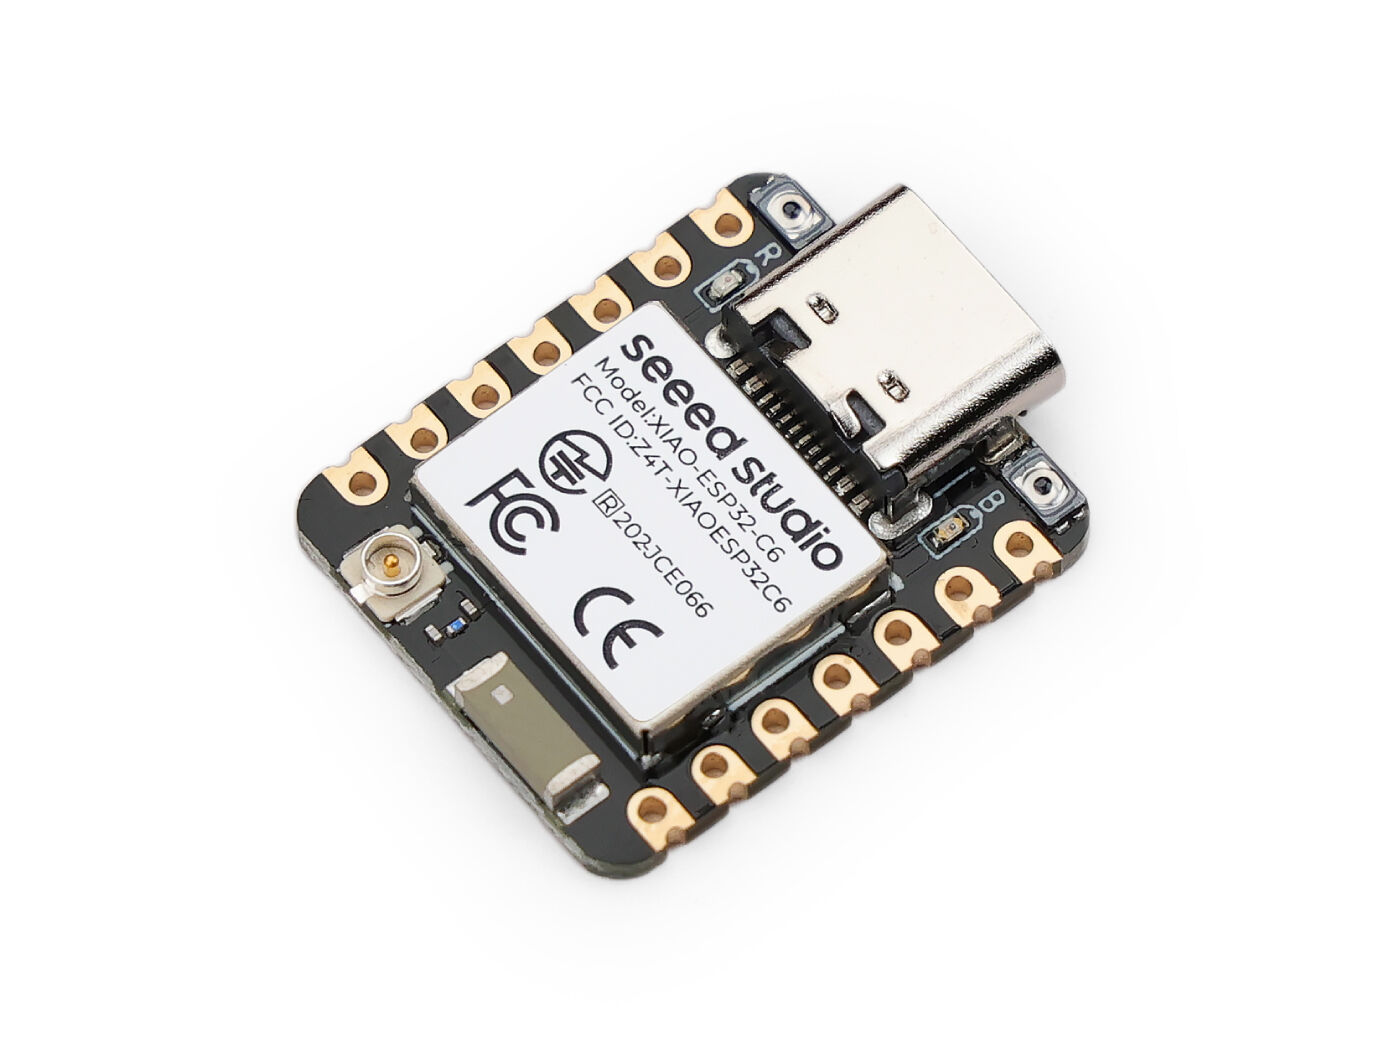
\includegraphics[width=20mm]{./Imagenes/Módulo1/Microcontrolador/1-113991254-seeedxiao-esp32c6-45font_1.jpg}\\
\hline
ESP32-C3 SuperMini \cite{K} & RISC-V 32-bit Single-Core / 160 MHz & ROM 400KB, SRAM 400KB, Flash 4MB & Wi-Fi 4 (802.11n), BLE 5 & 2xUART, 2xI2C, 1xSPI, 13xGPIO & 3.3V (5V VCC) & \$100-200 &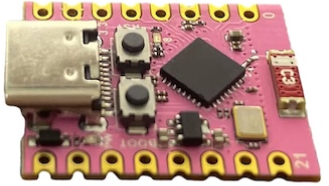
\includegraphics[width=20mm]{./Imagenes/Módulo1/Microcontrolador/c3_mini.png} \\
\hline
ESP32-C6-DEVKITC-1-N8 \cite{zotero-item-62}& RISC-V 32-bit Single-Core / 160 MHz & ROM 320KB, SRAM 512KB, Flash 8MB & Wi-Fi 6, BLE 5, Zigbee 3.0, Thread & 4xSPI, 3xUART, 2xI2C, 2xI2S, 23xGPIO & 3.3V (5V Micro-USB) & \$160-250 & 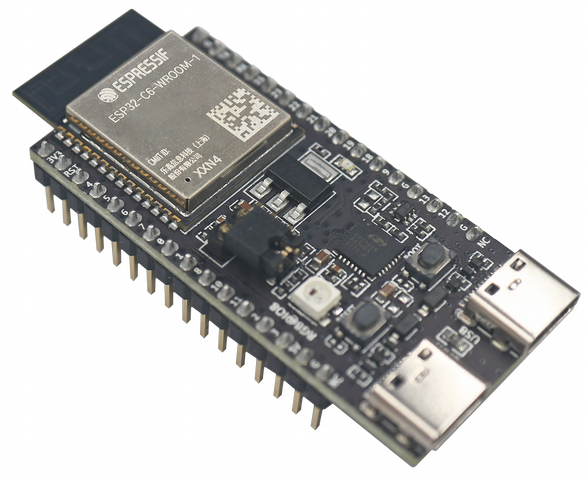
\includegraphics[width=20mm]{./Imagenes/Módulo1/Microcontrolador/esp32-c6.png}\\
\hline
ESP32-DevKitC-32E \cite{Embajadores} & Xtensa LX6 Dual-Core / 240 MHz & ROM 448KB, SRAM 520KB, Flash 4MB & Wi-Fi 4 (802.11n), BT 4.2 & 3xSPI, 3xUART, 2xI2C, 2xI2S, 34xGPIO & 3.3V (5V Micro-USB) & \$160-250 & 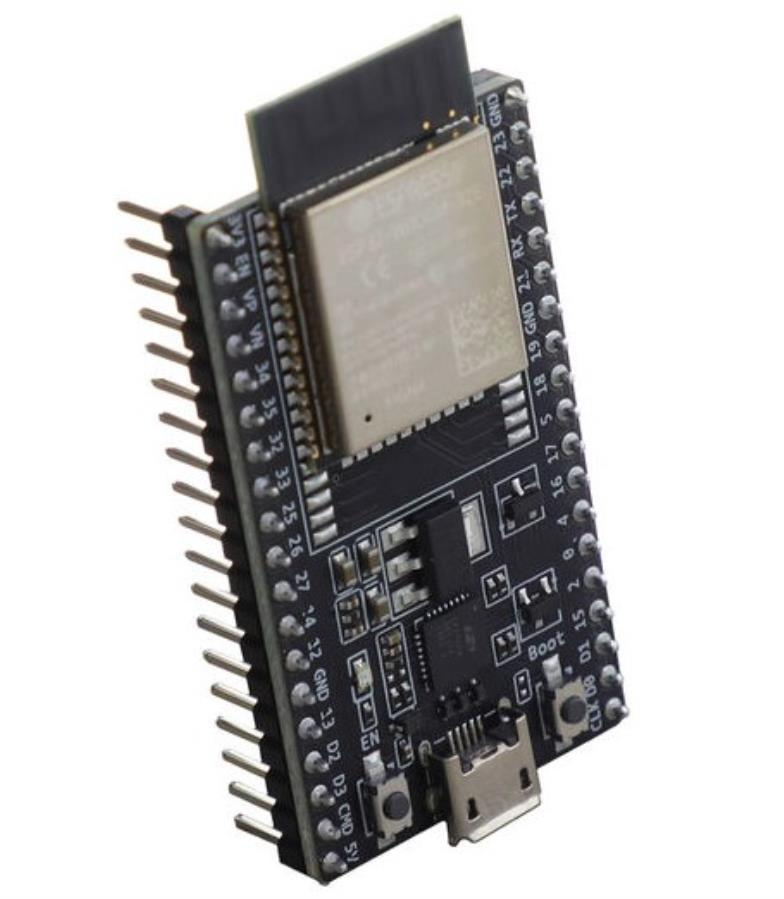
\includegraphics[width=20mm]{./Imagenes/Módulo1/Microcontrolador/esp32.jpg}\\
\hline
ESP32-C2 (Módulo) \cite{zotero-item-66}& RISC-V 32-bit Single-Core / 120 MHz & ROM 320KB, SRAM 272KB, Flash 4MB & Wi-Fi 4 (802.11n), BLE 5 & 2xSPI, 2xUART, 1xI2C, 1xI2S, 14xGPIO & 3.3V & \$120-250 & 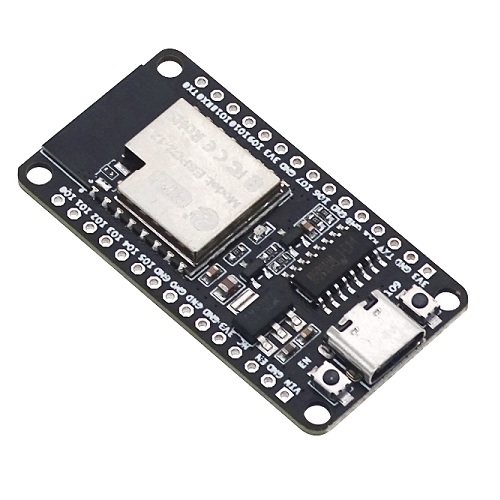
\includegraphics[width=20mm]{./Imagenes/Módulo1/Microcontrolador/c2.jpg}\\
\hline
Raspberry Pi Pico 2 W \cite{zotero-item-68}& ARM Cortex M0+ Dual-Core / 133 MHz & SRAM 264KB, Flash 4MB & Wi-Fi 4 (802.11n), BT 5.2 & 2xSPI, 2xI2C, 2xUART, 16xPWM, 26xGPIO & 3.3V (5V Micro-USB) & \$200-280 & 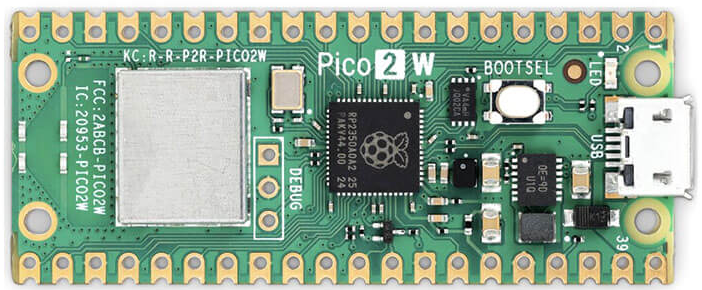
\includegraphics[width=20mm]{./Imagenes/Módulo1/Microcontrolador/pi2.png}\\
\hline
\end{longtable}
\endgroup
\end{landscape}



